\chapter{Introdução}

\section{Motivação}
Há uma expectativa de que o número de casas inteligentes aumente cerca de 17\% nos Estados Unidos no ano de 2017 \cite{mckinseyReport}, onde já se tem investimentos de grandes empresas, como Google, Amazon e Apple, mostrando a relevância do tema no momento atual. O interesse nessa área é tamanho que a Google investiu cerca de 5 milhões de dólares em um comercial de seu produto Google Home no Super Bowl 2017 (final de futebol americano nos EUA) \cite{kennemer}.

Assim, as oportunidades trazidas pelo conceito de Internet das Coisas à área de automação residencial são uma grande motivação para esse projeto. Também destacam-se as possibilidades de trazer tais tecnologias de casas inteligentes ao mercado nacional, personalizando produtos e adequando-as às necessidades dos potenciais consumidores brasileiros. Mesmo nos Estados Unidos, ainda é necessário algum tempo até que a casa conectada se consolide, de modo que há grandes oportunidade de pioneirismo no mercado brasileiro, com o lançamento de produtos de casa conectada a preços acessíveis e focando nas necessidades dos consumidores locais.

\section{Projeto Hedwig}

\subsection{Objetivo}
A contribuição do projeto será um sistema baseado em arquitetura local modularizada, com funcionalidades local e em nuvem, e provedor de uma API que permita seu acesso por diversos clientes - como \textit{websites} ou aplicativos para \textit{smartphones} - e que seja capaz de monitorar e agir em diversos módulos presentes na residência do usuário final do sistema. Ainda irá dispor de \textit{Machine Learning}, inicialmente alimentado com dados reais de quatro módulos exemplo, armazenados em nuvem, o que irá permitir adaptabilidade do sistema à utilização por cada um de seus usuários.

Desta forma, os principais pontos do projeto são:

\begin{itemize}
\item \textbf{Robustez}

3 níveis de funcionamento: Online, Local e Offline, para garantir a disponibilidade mesmo com problemas (queda do servidor, internet indisponível, falha no roteador), com medidas como tentativa automática de reconexão, monitoramento e manutenções preventivas e corretivas do sistema.

\item \textbf{Modularidade}

Garante a independência de funcionamento dos módulos que atendem às várias necessidades, contribuindo para a robustez. Diminui o custo e personaliza o produto, de acordo com as necessidades do cliente.

\item \textbf{Machine Learning}

Levantamento de rotinas para gerar conhecimento, que se mostra como notificações, alertas e acionamentos automáticos de funções para o cliente.

\item \textbf{Segurança}

Autenticação dos usuários e proteção contra ataques de DoS (\cite{Denial of Service}) Local.
\end{itemize}


\begin{figure}[H]
	\centering
	\caption{Projeto Hedwig}
  
\includegraphics[width=0.2\textwidth]{hedwigLogo}
\label{fig:hedwigLogo}
\end{figure}

\subsection{Nome do Projeto}
O nome do projeto foi escolhido em homenagem a Hedy Lamarr. Nascida Hedwig Eva Maria Kiesler \cite{shearer}, a atriz e inventora desenvolveu, durante a Segunda Guerra Mundial, um aparelho de interferência em rádio para despistar radares nazistas, cujos princípios estão incorporados nas tecnologias atuais de Wi-fi, CDMA e Bluetooth \cite{electronicFrontier}. Baseado nessa ideia de um sistema de comunicação seguro, e como reconhecimento de seu trabalho, foi dado esse nome ao projeto aqui descrito.

\section{Aplicações}
Como aplicações do projeto Hedwig, destacam-se a automação de eletrodomésticos e iluminação, segurança no acesso à casa, economia nas contas de água e energia elétrica, além de um monitoramento remoto de pessoas que moram sozinhas (como é o caso de idosos), garantindo a tranquilidade de seus familiares e mantendo a segurança do indivíduo.

Exemplos de módulos que podem ser incluídos no sistema são: quarto (despertador, iluminação, monitoramento de temperatura e umidade); cozinha (timer, iluminação, monitoramento de presença e gás); acesso (controle de abertura, monitoramento de estado); externo (monitoramento de temperatura, umidade, energia elétrica e consumo de água); corredor (monitoramento de presença, iluminação), chuveiro (controle de temperatura/potência a partir do perfil de usuário e temperatura externa) e ar condicionado (controle da potência a partir do monitoramento das temperaturas interna e externa da casa).

\subsection{Aplicações de Machine Learning}
Como possíveis perguntas a serem respondidas pelo módulo de Machine Learning do projeto e os dados a serem coletados (em diferentes lugares da casa), temos:

\begin{itemize}
\item Quando notificar a chegada de pessoas ou falta dela? - presença e sensor de abertura do portão
\item Quando enviar alertas de atividade suspeita? - presença
\item Quanto o sistema é usado? (Por funcionalidade) - sensor de abertura e log de aberturas pelo módulo
\item Quando notificar condições insalubres, como temperatura e umidade altas persistentes? - temperatura e umidade
\item Quando notificar falta de atividades rotineiras (como acordar, almoçar) - presença
\item Melhor horário para despertar? - presença
\item Notificar mudança brusca de temperatura, principalmente esfriamento? - temperaturas interna e externa, umidade (para sensação térmica)
\item Quanto o sistema está indisponível na instalação do cliente? - log de qualquer dado periódico
\item Quando acender ou apagar a luz? - presença, acionamento manual (horário e módulo)
\item Quantas vezes notificar? Prioridades? - respostas do cliente (log), para notificar o mínimo necessário, e classificação de notificações (email, somente quando usuário abre o aplicativo, notificação no celular e até módulo de painel externo com buzzer, no caso de comunicação de situação de perigo entre residências fisicamente separadas).
\end{itemize}

Respondendo a essas perguntas, esperamos contribuir para a construção de um sistema autônomo, que aprende com feedbacks do usuário seja pelo monitoramento por módulos ou respostas dadas pelo aplicativo, atuando em segurança (safety), saúde e A
automação da residência do cliente.

\subsection{Módulo de Acesso}
Buscando garantir mais segurança e comodidade para o acesso à residência, além de um controle de liberação, o módulo de acesso atua em paralelo com uma fechadura eletrônica, que é acionada por meio de um controle por ondas de rádio, para que, mesmo com falha total do sistema, o usuário possa abrir o portão (ou que ele possa optar por usar o antigo sistema exclusivamente).

\begin{figure}[H]
	\centering
	\caption{Diagrama ilustrativo do módulo de Acesso ao Portão}
  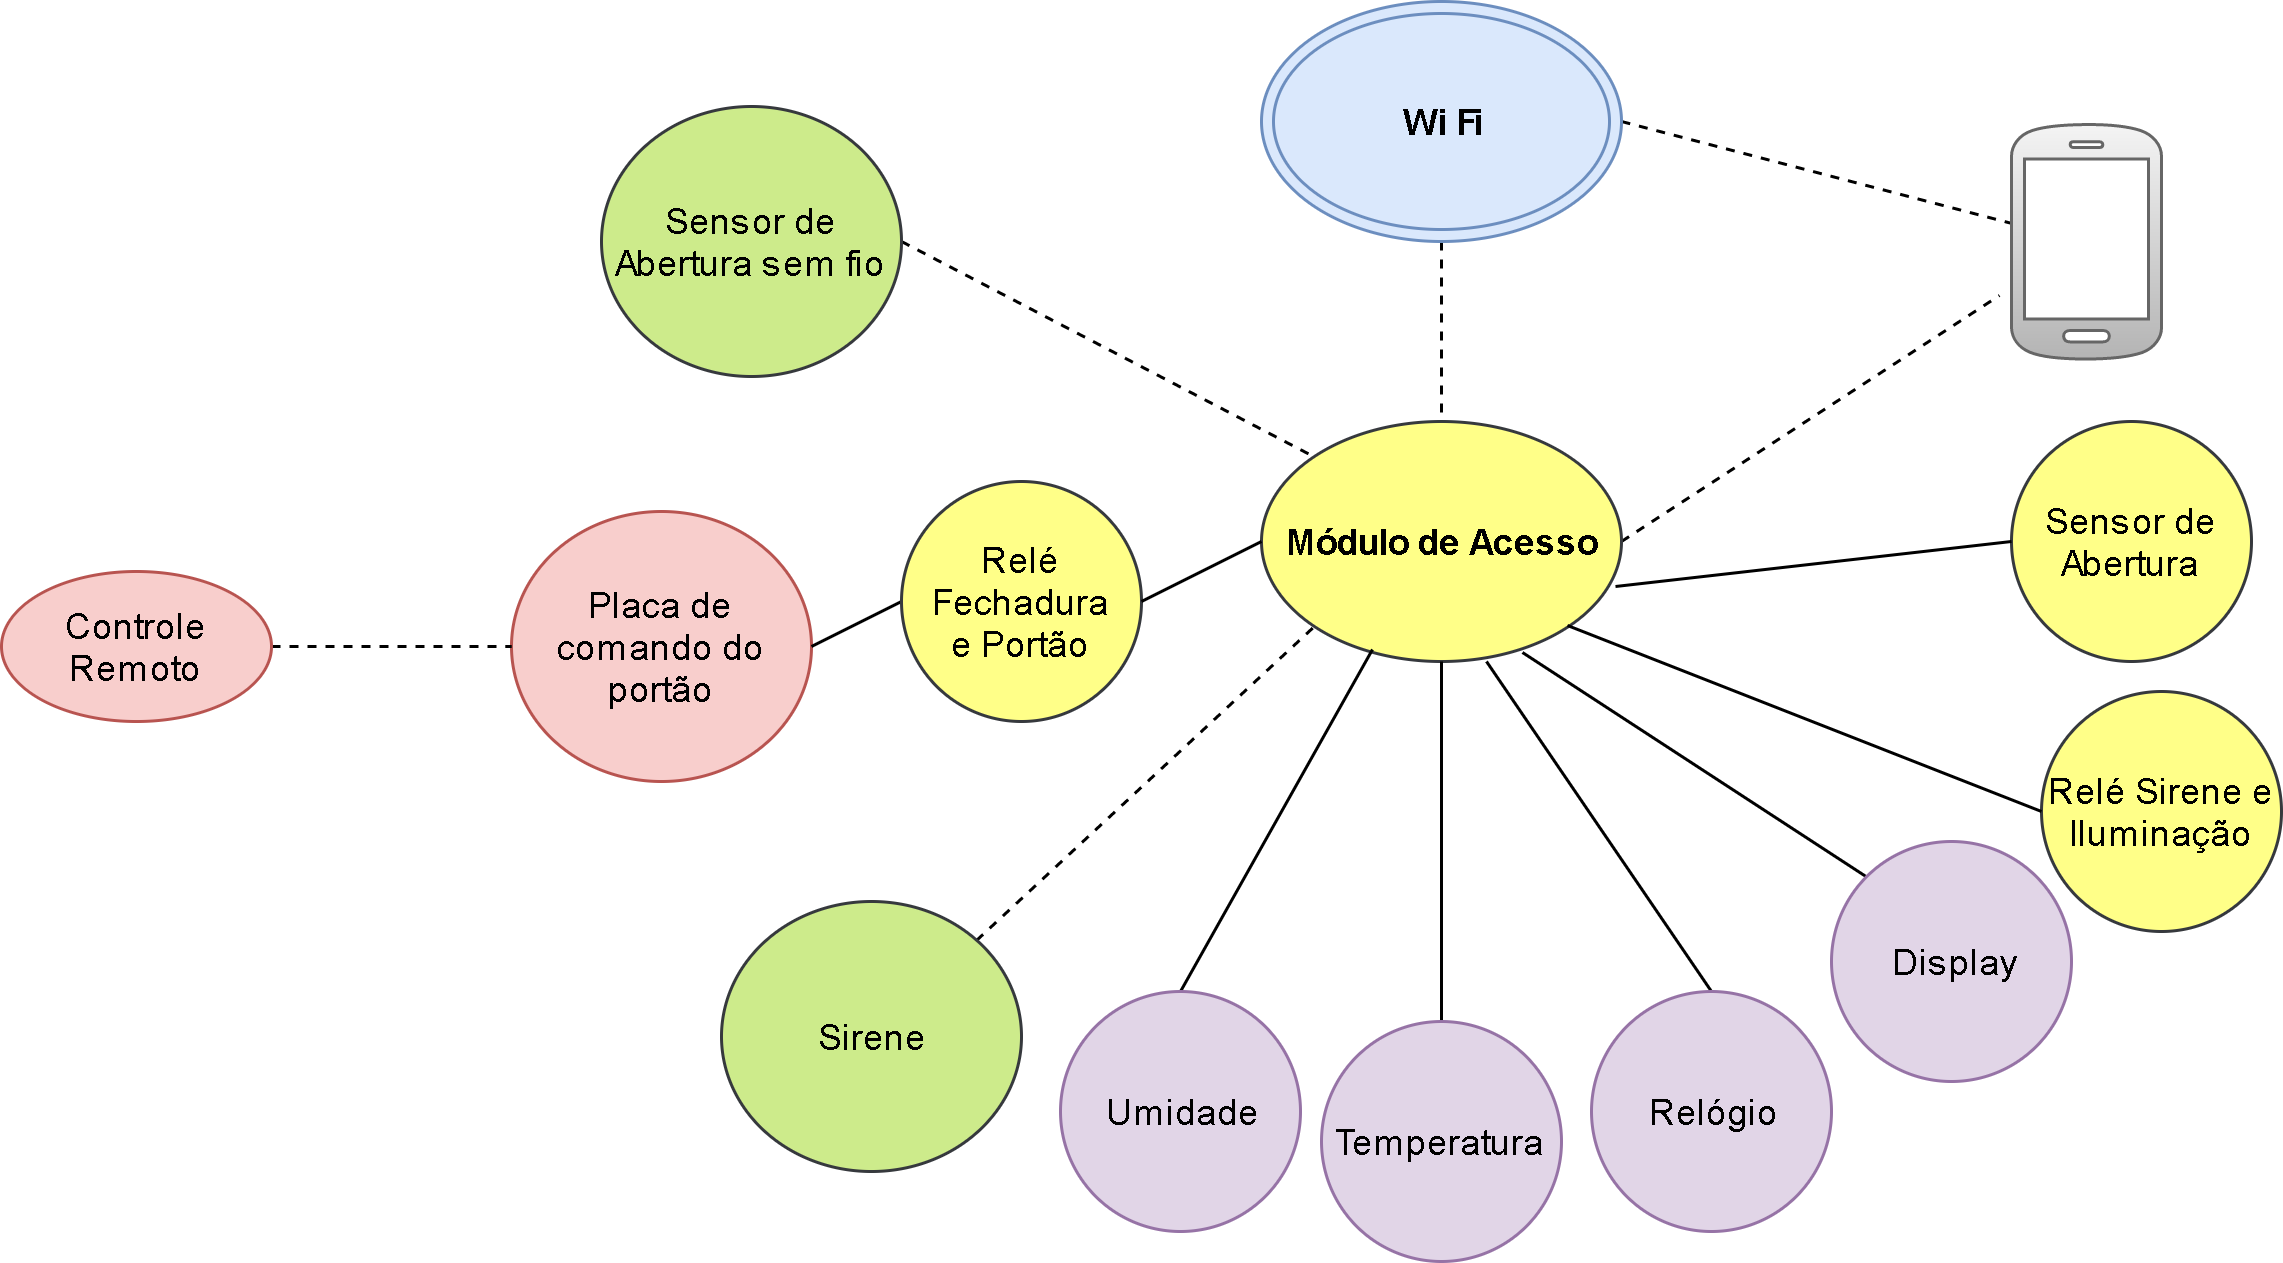
\includegraphics[width=0.8\textwidth]{diagramaModuloAcesso}
\label{fig:diagramaModuloAcesso}
\end{figure}

O diagrama ilustra o sistema já existente (em vermelho), sensor e sirene sem fio adicionais em verde (dispositivos externos ao módulo, que se comunicam por rádio), o próprio módulo de acesso, com um buzzer embutido, e sua conexão com a rede local Wi-Fi ou sua conexão direta com o celular (quando o módulo opera como um ponto de acesso de rede) em amarelo, além de funcionalidades adicionais em roxo.

A comodidade está em abrir o portão por meio do celular, por um aplicativo ou página web local, sem a necessidade de carregar uma chave ou controle. Além disso, pode prover maior praticidade (enquanto o celular está com o usuário na maioria do tempo, chave e controle podem estar na mochila). Para usuários que fazem passeios a pé, em sua maioria curtos, ou que vão à academia perto de suas casas, carregar chaves/controles é particularmente incômodo.

Por outro lado, é desejável realizar esse controle de forma segura. Por isso, o acesso é apenas local (o usuário deve estar com o celular conectado à rede local para acessar a página local, por exemplo), e um algoritmo de rotação de teclas é realizado, para evitar que pessoas mal intencionadas possam (1) olhar e copiar a senha que o usuário digita em seu celular e (2) copiar os dados de abertura e usá-los mais tarde (“middle man”). Na última alternativa, a cada acesso de um usuário, um novo mapeamento de teclas é gerado e enviado ao usuário. Mesmo que haja cópia, ela não funcionará devido ao mapeamento ter mudado. Observe ainda que a fechadura eletrônica por si só já estava vulnerável a isso (há inclusive dispositivos copiadores de senhas).

Outro aspecto de segurança é a preocupação dos usuários com o estado do portão. Muitas vezes, pode haver esquecimento ou falha e o portão ficar aberto. Para mitigar esse perigo, o módulo deve monitorar, por meio de um sensor, o estado da porta (aberto/fechado), e alertar localmente (por meio de “buzzer”) e remotamente (por email ou notificação no \texit{smartphone}, por exemplo) o usuário a abertura em horários . Essa e outras configurações (como de rede) são acessadas por meio de uma senha diferente daquela de abertura, para que a interface básica seja simples para uso.

Para o caso de falha de envio de email (servidor falha, ou algum outro problema), há um algoritmo de novas tentativas com tempos progressivamente maiores conforme as falhas ocorrerem, que busca deixar o módulo disponível para outras funções enquanto o serviço de e-mail não está disponível. No caso de indisponibilidade da internet, temos um procedimento análogo.

Para o caso de falta de conexão à internet, o módulo não seria controlável pela API, e as atualizações de dados como estado do portão seriam armazenadas para serem enviadas ao servidor em momento posterior, quando houvesse conexão à internet novamente. Caso o usuário esteja conectado à mesma rede local que o módulo, o mesmo continuaria funcionando normalmente.

Já no caso de falha da rede local, ou desconexão do módulo da rede local por problema de autenticação ou outros, o módulo de acesso ativa o \texit{Access Point}, e possibilita ao usuário acessar a rede do módulo e abrir o portão.

% TODO (victor) checar esse parágrafo abaixo. Acho que não ficou claro o que é esse "travamento"
Para evitar o travamento, um sinal de “keep alive” é monitorado, e um circuito anti travamento deve ativar um “hard reset” (reset por hardware), ou então uma rotina de “soft reset” deve ser acionada. No entanto, observe que a segunda alternativa é a mais fácil de implementar, mas a menos robusta, já que ainda pode não funcionar em casos de loop infinito.

% TODO (victor) não entendi a parte do "executa algoritmo análogo ao do envio de emails"
Outra situação que poderia gerar indisponibilidade do sistema é um ataque de DoS local (“Evil Twin”), no qual uma rede mal intencionada usa o mesmo SSID (\texit{Service Set Identifier}, o nome associado à rede WLAN) da rede original, tentando obter a senha na ocasião de reconexão de módulos. Muitas vezes, é também acompanhado de rádio interferência e outros procedimentos para fazer os módulos se desconectarem. Para mitigar o risco, cada módulo tenta inicialmente se conectar usando uma senha falsa no SSID fornecido. Caso obtenha sucesso (se a rede for aberta, como é o caso na maioria desses ataques), ele executa algoritmo análogo ao envio de emails (observe que enquanto não está conectado à rede o módulo atua como ponto de acesso e disponibiliza funcionalidades básicas). Caso ele não obtenha sucesso usando a senha errada (portanto, não detectou a situação de “evil twin”), o módulo envia a senha correta. Para proteger a rede, um controlador local do sistema pode atuar junto ao roteador e desligar a conexão sem fio enquanto a situação se manter.

O controle de acesso pode ser implementado por meio de persistência de dados de login e senha, e o uso de diversas senhas para uma residência (uma para cada morador - isso torna possível o conhecimento dos usuários que abriram o portão sem a necessidade de login prévio, facilitando o uso). O log destes acessos pode ser analisado (utilizando técnicas de Machine Learning) para determinar perfis de acesso, e evoluir até o sistema saber quando houver um acesso em horário inesperado e notificar o usuário remotamente. O aprendizado de máquina é fundamental aqui para descobrir comportamentos que podem ser entendidos como suspeitos. Para um usuário que costuma chegar em um horário aproximado todos os dias, e acionar funções semelhantes da casa, uma tentativa de acesso que não se enquadre em tais padrões pode ser produto de atividade criminosa, a qual pode ser informada pela casa para uma central, que acionará a polícia caso não seja um falso positivo.
